\section{基本概念}{

\subsection{六大基本初等函数}{
    常数函数,幂函数,指数函数,对数函数,三角函数
}%六大基本初等函数结尾

\subsection{介值定理}{

在数学分析中,介值定理(英语:intermediate value theorem,又称中间值定理)描述了连续函数在两点之间的连续性:

假设有一连续函数$\fint:[a,b]\rightarrow \mathbf{R}$, 且假设$\fint(a)<\fint(b)$, 若对任意数$u$满足$\fint(a)<u<\fint(b)$,则存在一点$c,a<c<b$,使得$\fint(c) = u$,当$\fint(a)>\fint(b)$时也有类似叙述

直观的比喻:这代表在$[a,b]$区间上可以画出一条连续曲线,而不让笔离开纸面.
\newline

定理:

假设$I = [a,b]$是一个实数里的闭区间,而$f:I\rightarrow\mathbf{R}$是连续函数,那么其像集$\fint(I)$也是区间.他或者包含$[\fint(a),\fint(b)]$(如果$\fint(b)\leq\fint(a)$).换言之:

$\fint(I)\supseteq[\fint(a),\fint(b)]$.

或:

$\fint(I)\supseteq[\fint(b), \fint(a)]$.

介值定理通常以下述等价的形式表述:假设$f:I\rightarrow\mathbf{R}$是连续函数,且实数$u$满足$\fint(a)<u<\fint(b)$或$\fint(a)>u>\fint(b)$,则存在$c\in(a,b)$使得$\fint(c) = u$

\begin{center}
    图示:
    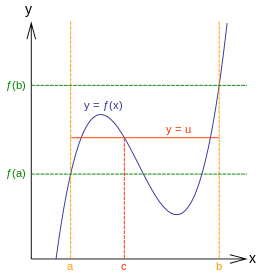
\includegraphics{resources/Intermediatevaluetheorem.png}
\end{center}
}%介值定理结尾

\subsection{二项式定理}{
    $(x + y)^n = x^n + \mathCombination{n - 1}{n}(x^{n-1} y) + \mathCombination{n - 2}{n}(x^{n-2} y^2) + \dots + y^n$

    \subsubsection{二项式系数与帕斯卡三角形(杨辉三角)}{

        二项式系数是二项式定理中各项的系数.一般而言,二项式系数由两个非负整数$n$和$k$作为参数来决定,写作$\begin{pmatrix}
                n \\
                k
            \end{pmatrix}$,定义为$(1 + x)^n$的多项式展开式中$x^k$项的系数,因此一定是非负整数.

        如果将二项式系数$\binom{n}{0},\binom{n}{1},\dots,\binom{n}{n}$写成一行,再依照$n = 0,1,2,3,...$顺序由上往下排列,则构成帕斯卡三角形(杨辉三角) :
        \begin{center}
            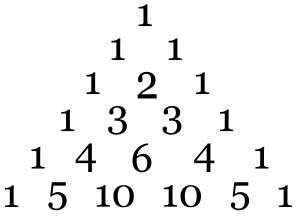
\includegraphics[scale=0.5]{resources/Pascal's_triangle_5.svg.png}
        \end{center}

        事实上,二项式系数就是排列组合中的组合 : ($\mathCombination{m}{n} \Longleftrightarrow \binom{m}{n}$)

        此外也有不同的表达方式 : $C(n,k),~_nC_k,~^nC_k,C^k_n,C^n_k\dots$

        %# TODO 看看Wiki : https://zh.wikipedia.org/wiki/%E4%BA%8C%E9%A0%85%E5%BC%8F%E4%BF%82%E6%95%B8
    }%二项式系数结尾

}%二项式定理结尾

\subsection{排列组合}{

    排列:$\mathPermutation{m}{n} = \cfrac{m!}{(m-n)!}$

    组合:$\mathCombination{m}{n} = \cfrac{\mathPermutation{m}{n}}{m!} = \cfrac{n!}{m!(n-m)!}$
}%排列组合结尾

\subsection{立方差公式}{
    \begin{itemize}
        \item $a^3 + b^3 = (a + b)(a^2 - ab + b^2)$
        \item $a^3 - b^3 = (a - b)(a^2 + ab + b^3)$
    \end{itemize}
}%立方差公式结尾

\subsection{等幂求和公式}{

}%等幂求和公式

\subsection{圆幂定理}{
    给定一个圆$r$及一点p,由p引出两条割线,分别于$r$相交于$A,B$及$C,D$,则有$PA \cdot PB = PC \cdot PD$

    事实上此定理包含三条定理 :

    \subsubsection{割线定理}{
        \begin{tikzpicture}
            \node (o) at (0.25,0.25){O};
            \draw [fill = black] (0,0) circle (1pt);
            \path[name path= c,draw] (0,0) circle (2);
            \node (B) at (-{sqrt(3)},1) {};
            \node (D) at (-{sqrt(3)},-1) {};
            \node (P) at (3,0){};
            \draw [fill = black] (P) circle (1pt);
            \draw [fill = black] (B) circle (1pt);
            \draw [fill = black] (D) circle (1pt);

            \path[name path = l1,draw] (B) node[above left]{$B$} -- (P) node [above right]{$P$};
            \path[name path = l2,draw] (D) node[below left]{$D$} -- (P);

            \node[name intersections = {of = c and l1,by=x}] (A) at (x){};
            \node[name intersections = {of = c and l2,by=x}] (C) at (x){};

            \draw [fill = black] (A) circle (1pt) node[above right]{$A$};
            \draw [fill = black] (C) circle (1pt) node[below right]{$C$};
        \end{tikzpicture}
        $PA \cdot PB = PC \cdot PD$
    }%割线定理结尾

    \subsubsection{交弦定理}{
        \begin{tikzpicture}
            \node (o) at (0.25,0.25){O};
            \draw [fill = black] (0,0) circle (1pt);
            \path[draw] (0,0) circle (2);
            \node (A) at (1,{sqrt(3)}){};
            \node (C) at ({-sqrt(3)},-1){};
            \node (D) at (2,0){};
            \node (B) at (0,-2){};
            \path[draw,name path = l1] (A) -- (B);
            \path[draw,name path = l2] (D) -- (C);
            \node[name intersections = {of = l1 and l2,by = x}] (E) at (x){};

            \draw [fill = black] (A) circle (1pt) node[above right]{$A$};
            \draw [fill = black] (B) circle (1pt) node[below]{$B$};
            \draw [fill = black] (C) circle (1pt) node[left]{$C$};
            \draw [fill = black] (D) circle (1pt) node[right]{$D$};
            \draw [fill = black] (E) circle (1pt) node[below right]{$E$};
        \end{tikzpicture}
        $EA \cdot EB = EC \cdot ED$
    }%交弦定理结尾

    \subsubsection{切割线定理}{
        \begin{tikzpicture}
            \node (o) at (0.25,0.25){O};
            \draw [fill = black] (0,0) circle (1pt);
            \path[name path= c,draw] (0,0) circle (2);

            \node (T) at (0,2){};
            \node (B) at ({-sqrt(3)},-1){};
            \node (P) at (5,2){};

            \draw (T) -- (P);
            \path[draw,name path = l1] (B) -- (P);

            \node[name intersections = {of = c and l1,by = x}] (A) at (x){};

            \draw [fill = black] (A) circle (1pt) node[above right]{$A$};
            \draw [fill = black] (B) circle (1pt) node[above left]{$B$};
            \draw [fill = black] (T) circle (1pt) node[above]{$T$};
            \draw [fill = black] (P) circle (1pt) node[right]{$P$};
        \end{tikzpicture}
        $PT^2 = PA \cdot PB$
    }%切割线定理结尾

}%圆幂定理结尾

\subsection{圆周角定理}{
    一条弧所对的圆周角$\alpha$等于所对圆心角的一半.

    \begin{tikzpicture}
        \node (o) at (0.25,0.25){O};
        \draw [fill = black] (0,0) circle (1pt);
        \path[name path= c,draw] (0,0) circle (2);
        \node (P1) at (-{sqrt(3)},1) {};
        \node (P2) at (-{sqrt(3)},-1) {};

        \draw (P1) -- (2,0) node[left]{$\alpha$} -- (P2);
        \draw (P1) -- (0,0) node[left]{$\beta$} -- (P2);

        \tikzPlaceDot{(P1)};
        \tikzPlaceDot{(P2)};
        \tikzPlaceDot{(2,0)};
    \end{tikzpicture}

}%圆周角定理结尾

\subsection{韦达定理}{
\subsubsection{韦达定理的普遍情况}{
设$P(x) = a_nx^n + a_{n-1}x^{n-1} + \dotsm + a_1x + a_0$是一个一元n次实(或复)系数多项式,首项系数$a_n \neq 0$,令P的n个根为$x_1,x_2,\dots,x_n$,则根$\{x_i\}$和系数$\{a_j\}$之间满足关系式 :

$$
    \begin{cases}
        x_1 + x_2 + \dotsm + x_{n-1} + x_n = -\cfrac{a_{n-1}}{a_n}                                                           \\
        (x_1x_2 + x_1x_3 + \dotsm + x_1x_n) + (x_2x_3 + x_2x_4 + \dotsm + x_2x_n) + \dotsm + x_{n-1}x = \cfrac{a_{n-2}}{a_n} \\
        \vdots                                                                                                               \\                                                                                                               \\
        x_1x_2 \dotsm x_n = (-1)^n\cfrac{a_n}{a_n}
    \end{cases}
$$

等价的说,对任何$k = 1,2,\dots,n$,系数比$\cfrac{a_{n-k}}{a_n}$是所有任取k个根的乘积的和的$(-1)^k$倍,即 :

$\sum\limits_{1 \leq i_1 < i_2 < \dotsm < i_k \leq n}x_{i_{1}}x_{i_{2}} \dotsm x_{i_{k}} = (-1)^k\cfrac{a_{n-k}}{a_n}$

其中$i_1 < i_2 < \dotsm < i_k$是要让所有根的组合都恰好出现一次.

(等号的左边被称作是初等对称多项式)
}%韦达定理的普遍情况结尾

\subsubsection{n = 2的情况(二次)}{
    设$x_1,x_2$是一元二次多项式$ax^2 + bx + c$的两根,则由$ax^2 +bx + c = a(x - x_1)(x - x_2) = ax^2 - a(x_1 + x_2)x + ax_1x_2$有 :

    $x_1 + x_2 = -\cfrac{b}{a},\qquad x_1x_2 = \cfrac{c}{a}$

    在这个情况下,韦达定理的逆定理同样成立 : 给定一个一元二次多项式$ax^2 + bx + c$,如果有两个数$x_1,x_2$,满足$x_1 + x_2 = -\cfrac{b}{a}$和$x_1x_2 = \cfrac{c}{a}$,则$x_1,x_2$就是多项式$ax^2 + bx + c$的两根.
}%n = 2的情况(二次)结尾

\subsubsection{n = 3的情况(三次)}{
    设$x_1,x_2,x_3$是一元三次多项式$ax^3 + bx^2 + cx + d$的三根,则

    $x_1 + x_2 + x_3 = -\cfrac{b}{a}, x_1x_2 + x_1x_3 + x_2x_3 = \cfrac{c}{a},x_1x_2x_3 = -\cfrac{d}{a}$
}%n = 3的情况(三次)结尾

}%韦达定理结尾

\subsection{极坐标}{
极坐标是不同于笛卡尔坐标系(直角坐标系)的另一种函数图像平面.

极坐标不同于笛卡尔坐标系,他没有x和y轴,而是用基准轴和角度表示一个点.

\subsubsection{极坐标系下的面积}{
    \begin{center}
        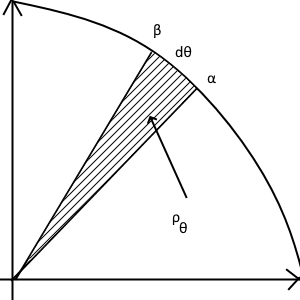
\includegraphics{resources/polar_coordness.png}
    \end{center}

    公式为$\cfrac{1}{2}\definiteIntegral{\beta}{\alpha}(p(\theta))^2d\theta$

    p是形成曲线的函数.
    }%极坐标下的面积结尾

    \subsubsection{转换公式}{
        从直角坐标系到极坐标有一套转换公式.

        $$
            \begin{cases}
                x = \rho\cos\theta \\
                y = \rho\sin\theta
            \end{cases}
        $$
    }%转换公式结尾

    \subsubsection{极坐标表示线}{
        \begin{center}
            \begin{tikzpicture}
                \draw (0,0) -- (0,5);
                \draw[->] (0,0) -- (5,0);
                \node (p1) at (1,4){(a,b)};
                \node (p2) at (3,1){(c,d)};
                \draw (p1) -- (p2);
            \end{tikzpicture}
        \end{center}

        由转换公式,可以将直线在直角坐标系下的解析式$y = kx + b$转换为在极坐标下的解析式 :
        $$
            \rho\sin\theta = k\rho\sin\theta + b
        $$
        再变形得到 :
        $$
            \rho = \cfrac{b}{\sin\theta - k\cos\theta}
        $$
    }%极坐标表示线结尾

    \subsubsection{极坐标表示面}{
        所谓"线动成面",想要用极坐标表示面,只需要加上$\rho$的取值条件就行(即 : $a \leq \rho \leq b$,此处的$a,b$也可以是关于其他变量的公式).
    }%极坐标表示面结尾

    \subsubsection{柱面坐标}{
        柱面坐标是一种将极坐标扩展到三维的方法,其实就是加了个z轴.因此转换公式为 :

        $$
            \begin{cases}
                x = \rho\cos\theta \\
                y = \rho\sin\theta \\
                z = z
            \end{cases}
        $$
    }%柱面坐标结尾

    \subsubsection{球面坐标}{
        球面坐标又是不同与柱面坐标的另一种形式,他引入了另一个表示角度的变量$\varphi$

        球面坐标由三个变量组成,如果将某一个点用向量$\vec{v}$表示,那么三个变量分别是 :
        \begin{itemize}
            \item $r$ : 表示$\vec{v}$的长度,可以理解成极坐标的$\rho$.取值范围为:$\left[0,+\infty\right)$
            \item $\theta$ : 用过原点以$z$轴作为法向量的平面作为极坐标的平面,$\vec{v}$投影到此平面上时$\theta$就是该投影在极坐标中的角度单位.取值范围为$\mediumBigCase{0,2\pi}$
            \item $\varphi$ : 以原点为顶点,$z$轴为旋转轴,$\vec{v}$作为母线的圆锥面的半顶角.也就是$\vec{v}$与$z$轴的夹角.取值范围为:$\mediumBigCase{0,\pi}$
        \end{itemize}

        从直角坐标系到球面坐标系的转换公式为 :
        $$
            \begin{cases}
                x = r\sin\varphi\cos\theta \\
                y = r\sin\varphi\sin\theta \\
                z = r\cos\varphi
            \end{cases}
        $$
    }%球面坐标结尾

}%极坐标结尾

\subsection{不等式}{

\subsubsection{基本不等式}{
    $\cfrac{a + b}{2} \geq \sqrt{ab}$

    注:当且仅当$a = b$时取等号

    其中$\cfrac{a+b}{2}$称为$a,b$的算数平均数,$\sqrt{ab}$称为$a,b$的几何平均数.

    将其变形,可得:
    \begin{enumerate}
        \item $a + b \geq 2\sqrt{ab}$(当且仅当$a = b$时取等号)
        \item $\cfrac{b}{a} + \cfrac{a}{b} \geq 2$($a,b$同号)
        \item $ab \leq (\cfrac{a + b}{2})^2$($a,b\in\mathRealNumberCollection$)
        \item $(\cfrac{a + b}{2})^2 \leq \cfrac{a^2 + b^2}{2}$($a,b\in\mathRealNumberCollection$)
    \end{enumerate}
}%基本不等式结尾


\subsubsection{柯西不等式}{
    柯西不等式有很多种形式:
    \begin{itemize}
        \item {
              二维形式:

              由$(a^2 + b^2)(c^2 + d^2)\geq(ac + bd)^2$变形:$ac + bd \leq \sqrt{(a^2 + b^2)(c^2 + d^2)}$

              当且仅当$ab = cd$(即$\cfrac{a}{c} = \cfrac{b}{d}$)时.

              一般形式为$\upDownSum{n}{i = 1}a_i^2\upDownSum{n}{i = 1}b_i^2\geq\bigCase{\upDownSum{n}{i = 1}a_ib_i)}^2$

              当$\cfrac{a_1}{b_1} = \cfrac{a_2}{b_2} = \dots = \cfrac{a_n}{b_n}$或$a_i,b_i,i = 1,2,3,\dots,n$中至少有一方全为$0$时等号成立.

              一般形式推广:$(x_1 + y_1 + \dots)(x_2 + y_2 + \dots)\dots(x_n + y_n + \dots) \geq \left[\bigCase{\upDownProd{n}{i = 1}x_i}^{\cfrac{1}{n}} + \bigCase{\upDownProd{n}{i = 1}y_i}^{\cfrac{1}{n}} + \dots\right]^n$

              此推广形式又称卡尔松不等式,其表述是:在m×n矩阵中,各列元素之和的几何平均不小于各行元素的几何平均之和.二维形式是卡尔松不等式n=2时的特殊情况.
              }
        \item {
              向量形式:

              对于内积空间中的向量$\vec{x}$和$\vec{y}$,有

              $|\innerProduct{\vec{x}}{\vec{y}}^2| \leq \innerProduct{\vec{x}}{\vec{x}} \times \innerProduct{\vec{y}}{\vec{y}}$

              其中$\innerProduct{\cdot}{\cdot}$表示内积.等价地,将两边开方,等式右边即可以写为两向量范数乘积的形式.

              $|\innerProduct{\vec{x}}{\vec{y}}| \leq ||\vec{x}||\cdot||\vec{y}||$.

              另外,当且仅当$x$和$y$线性相关时,等号成立(仅两个向量而言,线性相关等同于平行).

              若$x_1,\dotsm,x_n \in \mathConstant$和$y_1,\dotsm,y_n \in mathConstant$有虚部,内积即为标注内积.如果用上划线标记共轭复数,这个不等式可以更明确的表述为:

              $|\vec{x_1}\bar{\vec{y_1}} + \dotsm + \vec{x_n}\bar{\vec{y_n}}|^2\leq (|\vec{x_1}|^2 + \dotsm + |\vec{x_n}|^2)(|\vec{y_1}|^2 + \dotsm + |\vec{y_n}|^2)$.
              }
        \item {
              三角形式:

              在三角形$ABC$中,这个式子可以写作:$||\vec{AB}|| + ||\vec{BC}|| \geq ||\vec{AC}||$

              也就是说:$\sqrt{a^2 + b^2} + \sqrt{c^2 + d^2} \geq \sqrt{(a - c)^2 + (b - d)^2}$

              等号成立的条件为:$ad = bc,且ac + bc \geq 0$(即$\cfrac{a}{c} = \cfrac{b}{d}$).
              }
        \item {
              积分形式:

              $\bigCase{\int\defFunction{x}g(x)dx}^2 \leq \int\fint^2(x)dx \int g^2(x)dx$
              }
        \item {
              一般形式:

              设$V$是一线性空间,定义内积,记作$\innerProduct{\alpha}{\beta}$,则:

              $|\innerProduct{\alpha}{\beta}| \leq |\alpha||\beta|$.

              其中$\alpha,\beta$为$V$中的向量.
              }
    \end{itemize}
}%柯西不等式结尾

\subsubsection{均值不等式}{
平均数不等式,或称平均值不等式、均值不等式,是数学上的一组不等式,也是基本不等式的推广.它是说:

如果$x_{1},x_{2},\dotsm,x_{n}$是正数,则:

$\mathbf{H}_n \leq \mathbf{G}_n \leq \mathbf{A}_n \leq \mathbf{Q}_n$

其中:

$\mathbf{H}_n = \cfrac{n}{\upDownSum{n}{i = 1}\cfrac{1}{x_i}} = \cfrac{n}{\cfrac{1}{x_1} + \cfrac{1}{x_2} + \dotsm + \cfrac{1}{x_n}}$

$\mathbf{G}_n = \sqrt[n]{\upDownProd{n}{i = 1}x_i} = \sqrt[n]{x_1x_2\dotsm x_n}$

$\mathbf{A}_n = \cfrac{\upDownSum{n}{i = 1}x_i}{n} = \cfrac{x_1 + x_2 + x_n}{n}$

$\mathbf{Q}_n = \sqrt{\cfrac{\upDownSum{n}{i = 1}x^2_i}{n}} = \sqrt{\cfrac{x^2_1 + x^2_2 + \dotsm + x^2_n}{n}}$

当且仅当$x_1 = x_2 = \dotsm = x_n$,等号成立.

当$n = 2$时:

$\cfrac{2}{\cfrac{1}{x_1} + \cfrac{1}{x_2}} = \cfrac{2x_1x_2}{x_1 + x_2}\leq\sqrt{x_1x_2}\leq\cfrac{x_1 + x_2}{2}\leq\sqrt{\cfrac{x_1^2 + x_2^2}{2}}$

即对这些正数:调和平均数$\leq$几何平均数$\leq$算数平均数$\leq$平方平均数(方均根)

可简记为:“{\bfseries 算几调方}”
}%二元均值不等式结尾  

\subsubsection{算术-几何均值不等式}{
    算术-几何平均值不等式,简称算几不等式,是一个常见而基本的不等式,表现算术平均数和几何平均数之间恒定的不等关系.设$x_1,x_2,\dots,x_n$为$n$个正实数,他们的算数平均数是$\mathbf{A}_n = \cfrac{x_1 + x_2 + \dotsm + x_n}{n}$,他们的几何平均数是$\mathbf{G}_n = \sqrt[n]{x_1\cdot x_2 \dotsm x_n}$.算术-几何平均值不等式表明,对任意的正实数$x_1,\dotsm,x_n$,总有:

    \begin{center}
        $\mathbf{A}_n\geq\mathbf{G}_n$
    \end{center}

    等号当且仅当$x_1 = x_2 = \dotsm = x_n$时成立.

}%算术-几何均值不等式结尾

\subsubsection{常用不等式}{
    \begin{itemize}
        \item $a^2 + b^2 \geq \cfrac{1}{2}(a + b)^2$
        \item $a^2 + b^2 \geq 2ab$
        \item $ab \leq \cfrac{a^2 + b^2}{2}$
        \item $ab \leq (\cfrac{a + b}{2})^2$
        \item $a + b \geq 2\sqrt{ab}$
        \item $a + b \leq \sqrt{2(a^2 + b^2)}$
    \end{itemize}
}%常用不等式结尾

}%不等式结尾

\subsection{可微,可导,连续的关系}{

    \subsubsection{一元情况下的关系}{
        \begin{itemize}
            \item 可微是可导的充要条件,即:可微$\Leftrightarrow$可导
            \item 可微和可导都是连续的充分条件,即:可微$\rightarrow$连续、可导$\rightarrow$连续
        \end{itemize}

        \begin{center}
            \begin{tikzpicture}
                \node(a) at (0,1.5) {可微};
                \node(b) at (3,1.5) {可导};
                \node(c) at (1.5,0) {连续};
                \draw[<->] (a) -- (b);
                \draw[->] (a) -- (c);
                \draw[->] (b) -- (c);
            \end{tikzpicture}
        \end{center}
    }%一元情况下的关系结尾

    \subsubsection{多元情况下的关系}{
        \begin{itemize}
            \item 可微(全微分)是可导和连续的充分条件,即:可微$\Rightarrow$可导、可微$\Rightarrow$连续.
            \item 可导$\nRightarrow$连续.
        \end{itemize}

        \begin{center}
            一元 :
            \begin{tikzpicture}
                \node(a) at (0,1.5) {可微};
                \node(b) at (3,1.5) {可导};
                \node(c) at (1.5,0) {连续};
                \draw[->] (a) -- (b);
                \draw[->] (a) -- (c);
            \end{tikzpicture}
        \end{center}
    }%多元情况下的关系结尾

}%可微,可导,连续的关系结尾

\subsection{零散的定义}{
    \begin{enumerate}
        \item 有界:$\exists\epsilon,f(x) < \epsilon\quad(-\infty < x < \infty )$
        \item 什么时候函数能复合 : 内层值域$\in$外层定义域
    \end{enumerate}
}%零散的定义结尾

\subsection{零散的思想}{
    \begin{enumerate}
        \item 正变换是数学的重要工具,三角变换是只变其形不变其质的.三角变换常常先寻找式子所包含的各个角之间的联系,并以此为依据选择可以联系它们的适当公式,通过换元法把三角恒等变换问题转化为代数恒等变换问题.
    \end{enumerate}
}%零散的思想结尾

}%基本概念结尾